Mediante simulación realizar los siguiente cálculos:
\mkexercise{ Curva de transferencia $V_{out}-V_{in}$ en el
intervalo de tensiones de entrada $-5 \ V \leq V_{in}
\leq 5 \ V$ para el diodo D1N914 (Libreria DIODE.OLB)
utilizando el siguiente circuito:

\begin{figure}[H]
\centering
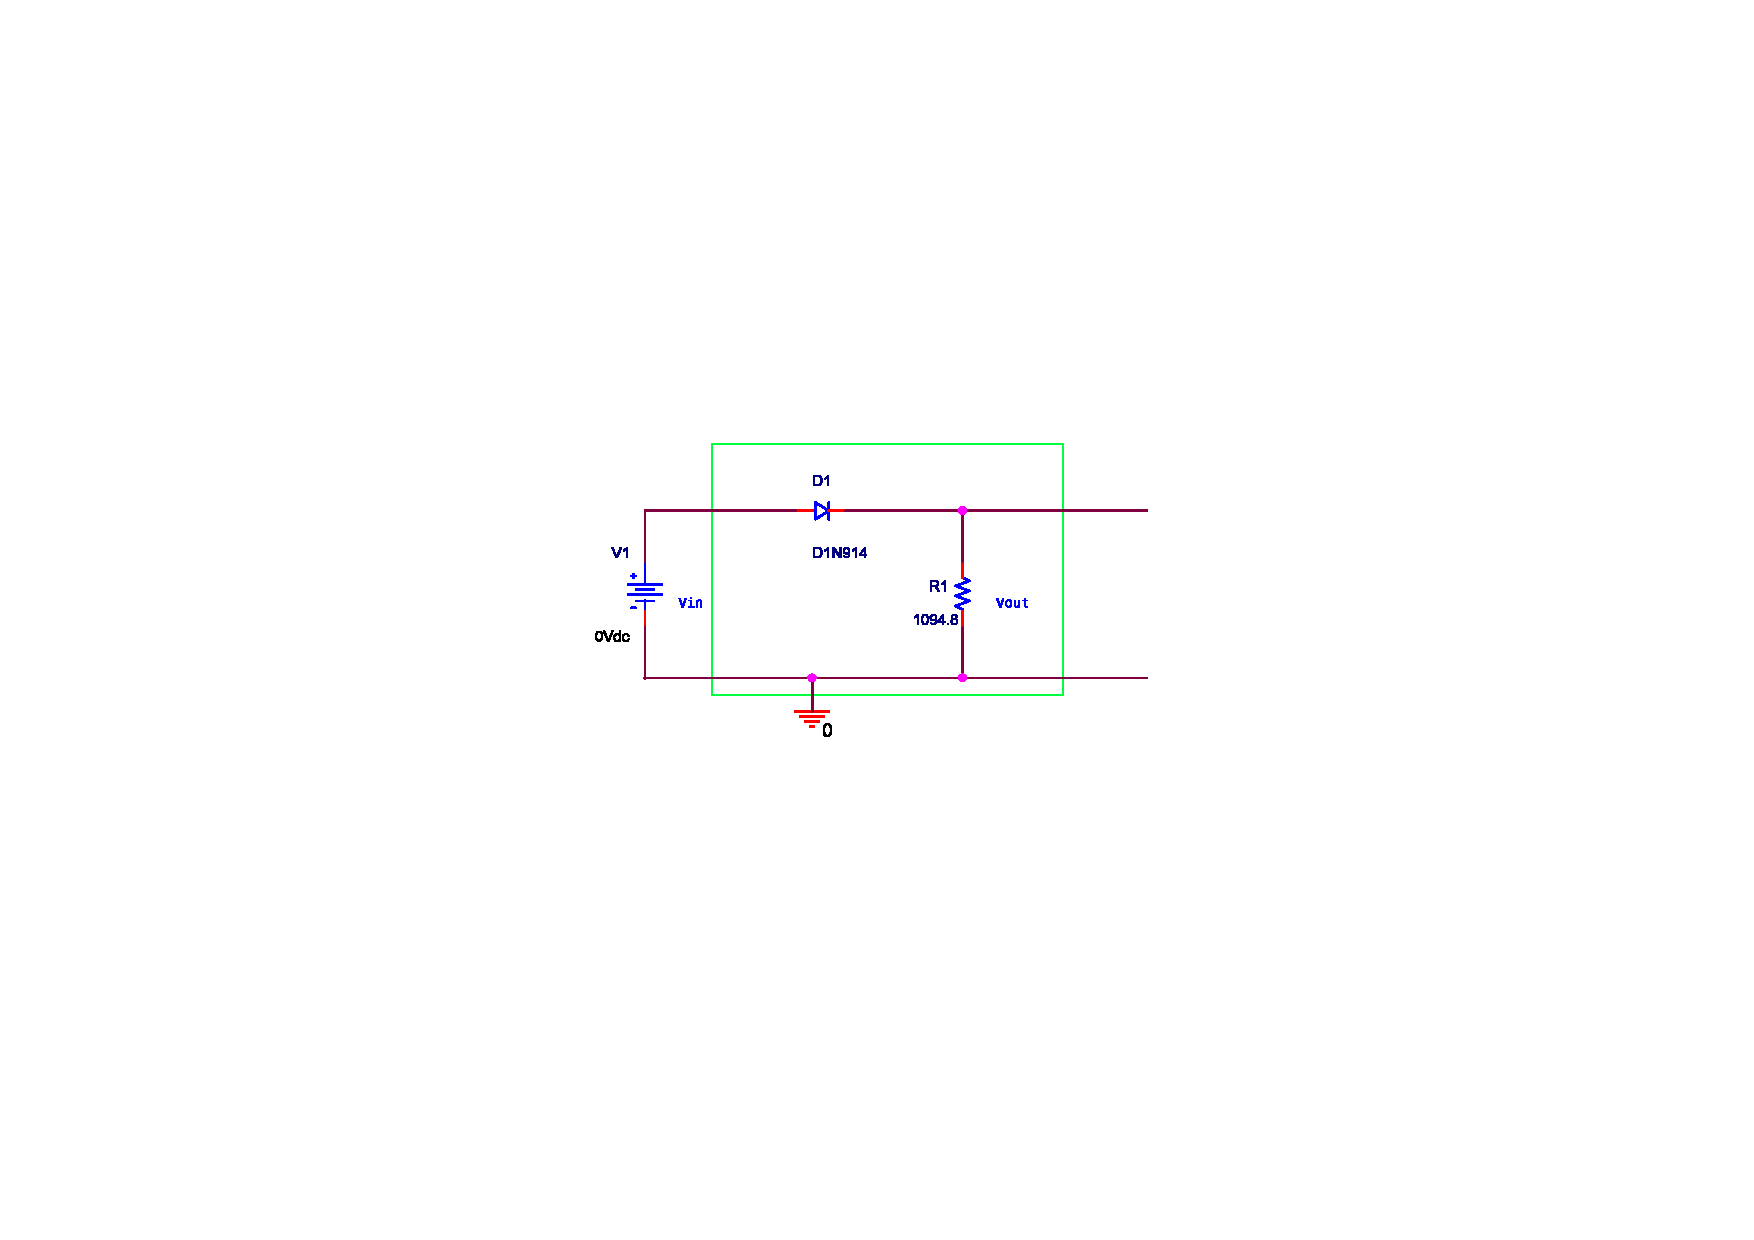
\includegraphics[clip, trim=10cm 8cm 10cm 7cm,
scale=0.90]{images/ejercicio_a.pdf}
% izquierda,abajo,derecha,arriba
\label{circuito_ejercicio_a}
\caption{Circuito de estudio ``a''}
\end{figure}

donde (DNI) se corresponde con las tres últimas cifras
(las numéricamente menos significativas), del DNI o
documento identificativo y el valor de la resistencia
$R_1 = 1000 + (DNI) * 0.1 \ \Omega$. Interpretar el
resultado teniendo en cuenta el modelo clásico de diodo
con pila y resistencia.}

\mksolution{
Para calcular la curva de transferencia del circuito tenemos que
representar la salida en función de la entrada, como el enunciado nos
pide usar el modelo diodo (ideal)-pila-resistencia obtenemos el
siguiente circuito de estudio.
La resistencia $R_d$ tiene un valor $10 \ \Omega $ para mA.

\begin{figure}[H]
\centering
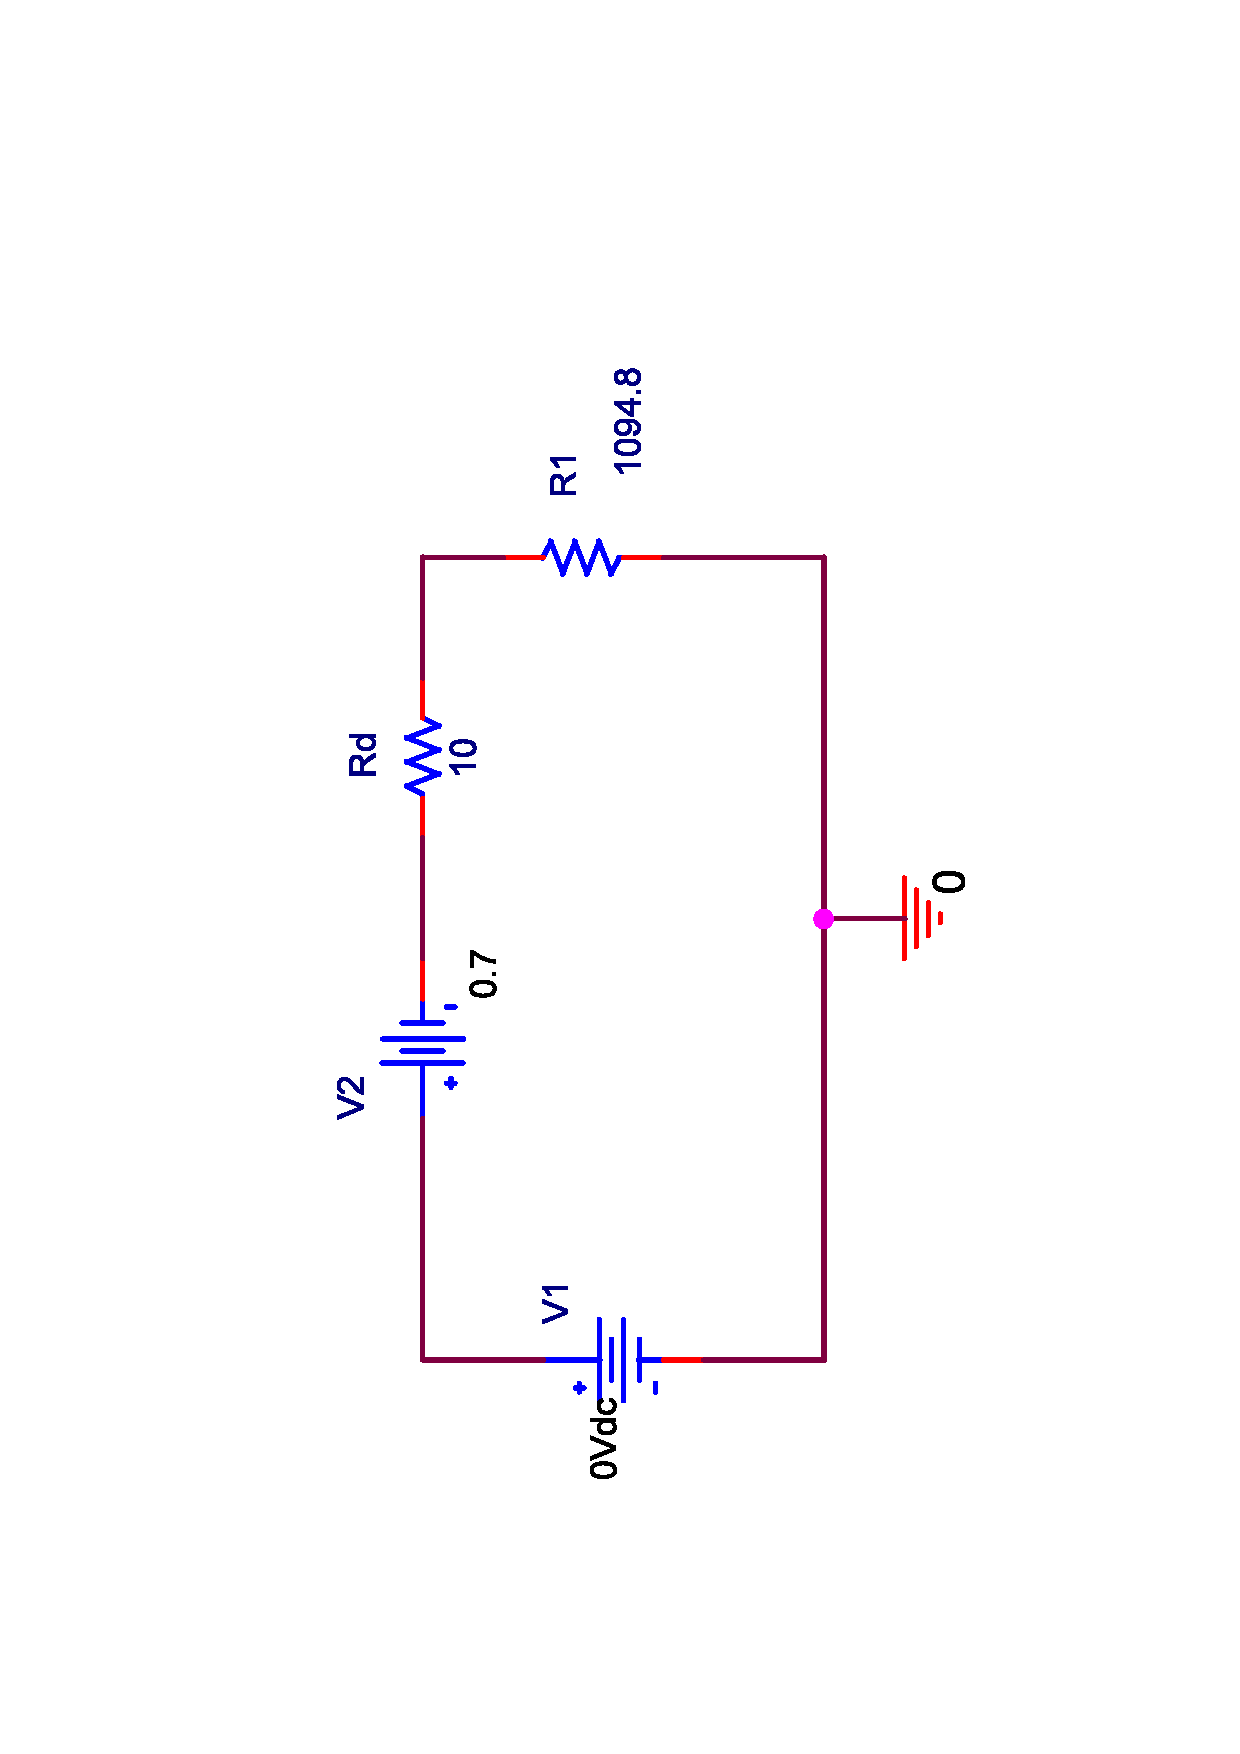
\includegraphics[clip, trim=5cm 5cm 4.5cm 6cm,
scale=0.50,angle=-90]{images/circuito_2.pdf}
\label{circuito_modelo_pila_resistencia}
\caption{Circuito con modelo pila resistencia}
\end{figure}

\begin{enumerate}[I)]
\item Zona de corte $V_{in}<0.7$

  La recta que representa la zona de no conducción es:
\begin{equation}
  y = 0 ,\  x \in (-5,\nc{7}{-1}) \ V
\end{equation}
\item Zona de conducción $V_{in}\geq 0.7$

Con las leyes de kirchhoff generamos las siguientes ecuaciones:
\begin{equation}
\begin{split}
0&=V_{in}-V_{d_{on}}-IR_D-IR_1\\
0&=Vout-IR_1\\
\end{split}
\end{equation}
Despejamos de la segunda ecuación $V_{out}$ y reemplazamos en la primera
    ecuación.
    \begin{equation}
        Vout = \dfrac{R_1\left(V_{in}-V_{d_{on}}\right)}{R_D+R_1}
    \end{equation}
    Si reemplazamos valores obtenemos la ecuación de la recta:
    \begin{equation}
      0.9909V_{in}-0.6936 = V_{out}
    \end{equation}
  \end{enumerate}

Con este resultado analítico podemos realizar una simulación y
comparar los resultados obtenidos.

\begin{figure}[H]
\centering
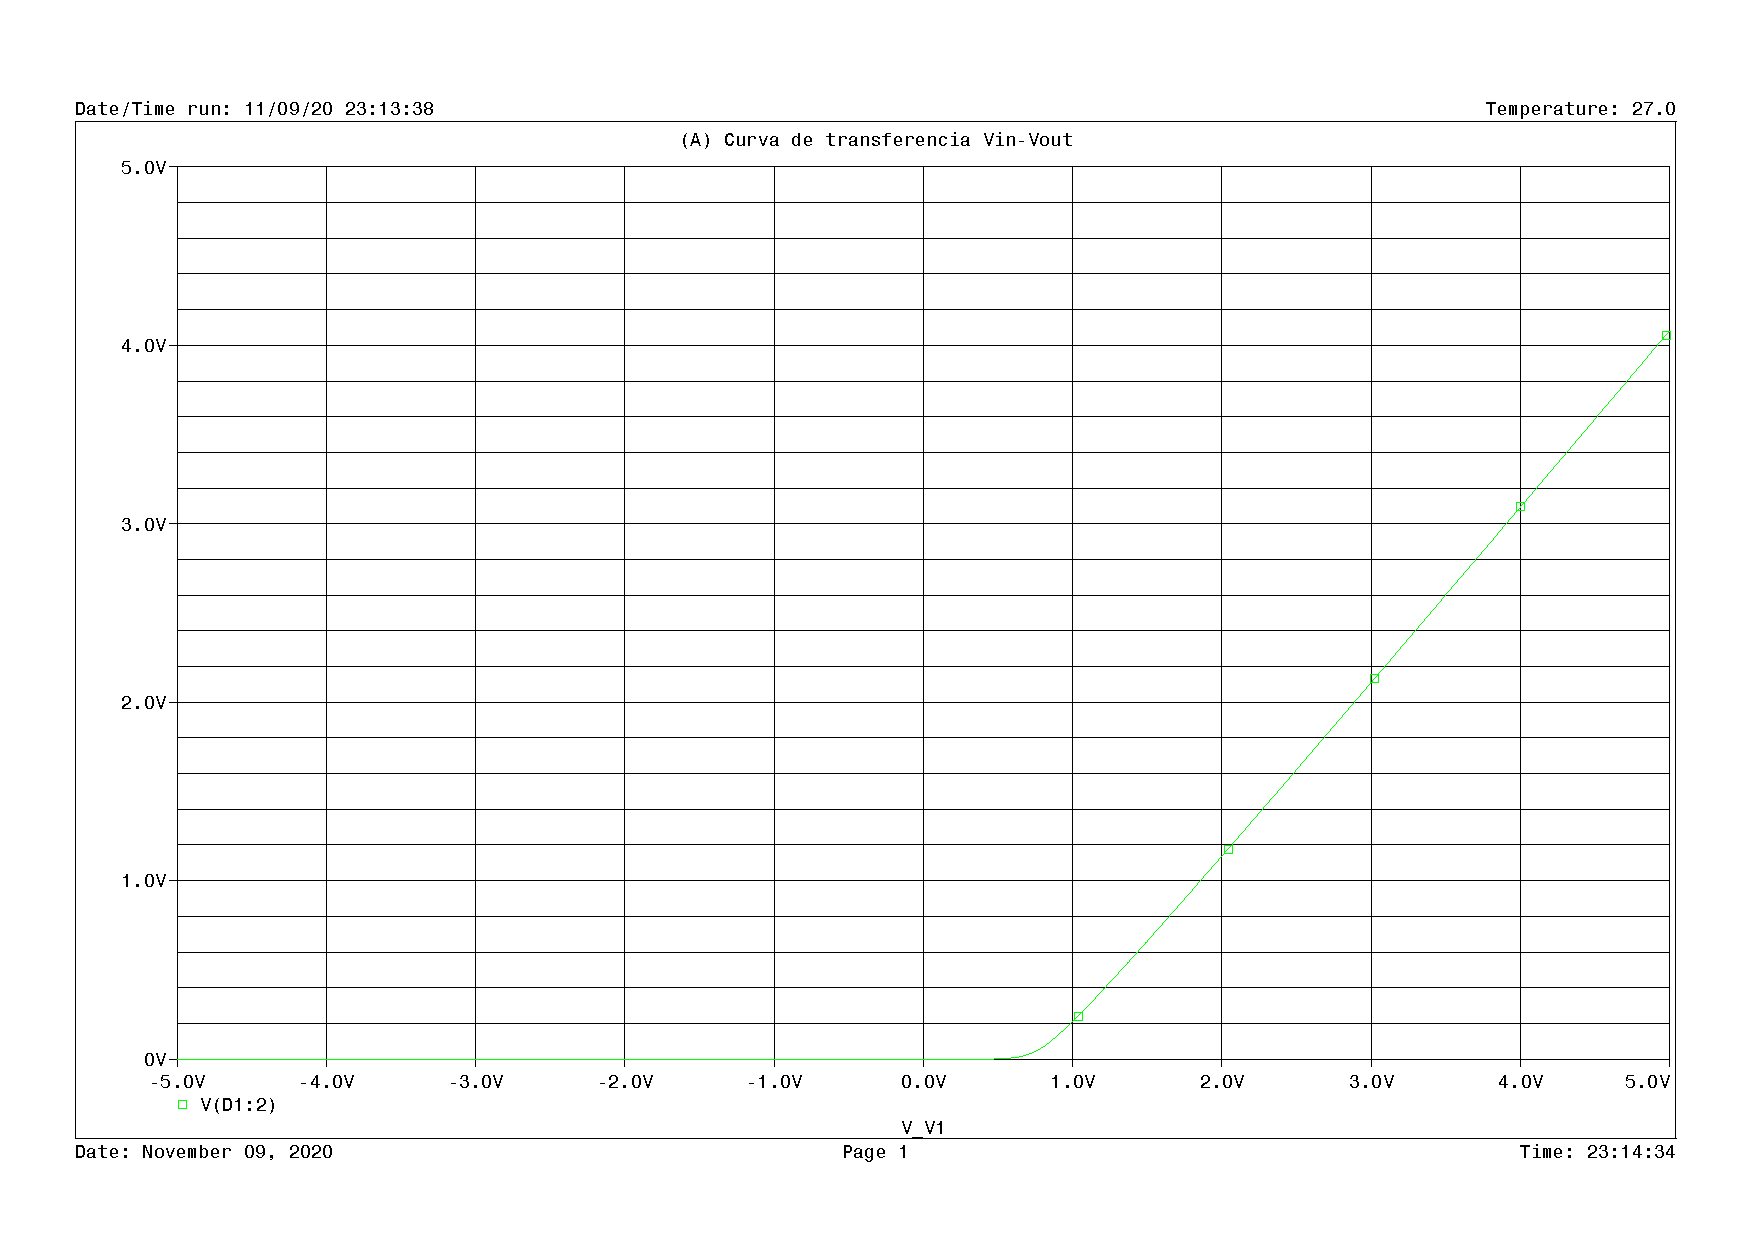
\includegraphics[scale=0.5]{images/puntuable_3_transfer.pdf}
\caption{Curva de transferencia del circuito
  \ref{circuito_ejercicio_a}}
\label{transfer_function_a}
\end{figure}

Se puede observar en la figura \ref{transfer_function_a} la
tensión de salida tiene dos tramos, la zona de conducción que
empieza en $0.7 \ V$ aprox. y la zona de no conducción.

Vamos a compararla con la recta obtenida analíticamente en la
siguiente gráfica.

\begin{figure}[H]
\centering
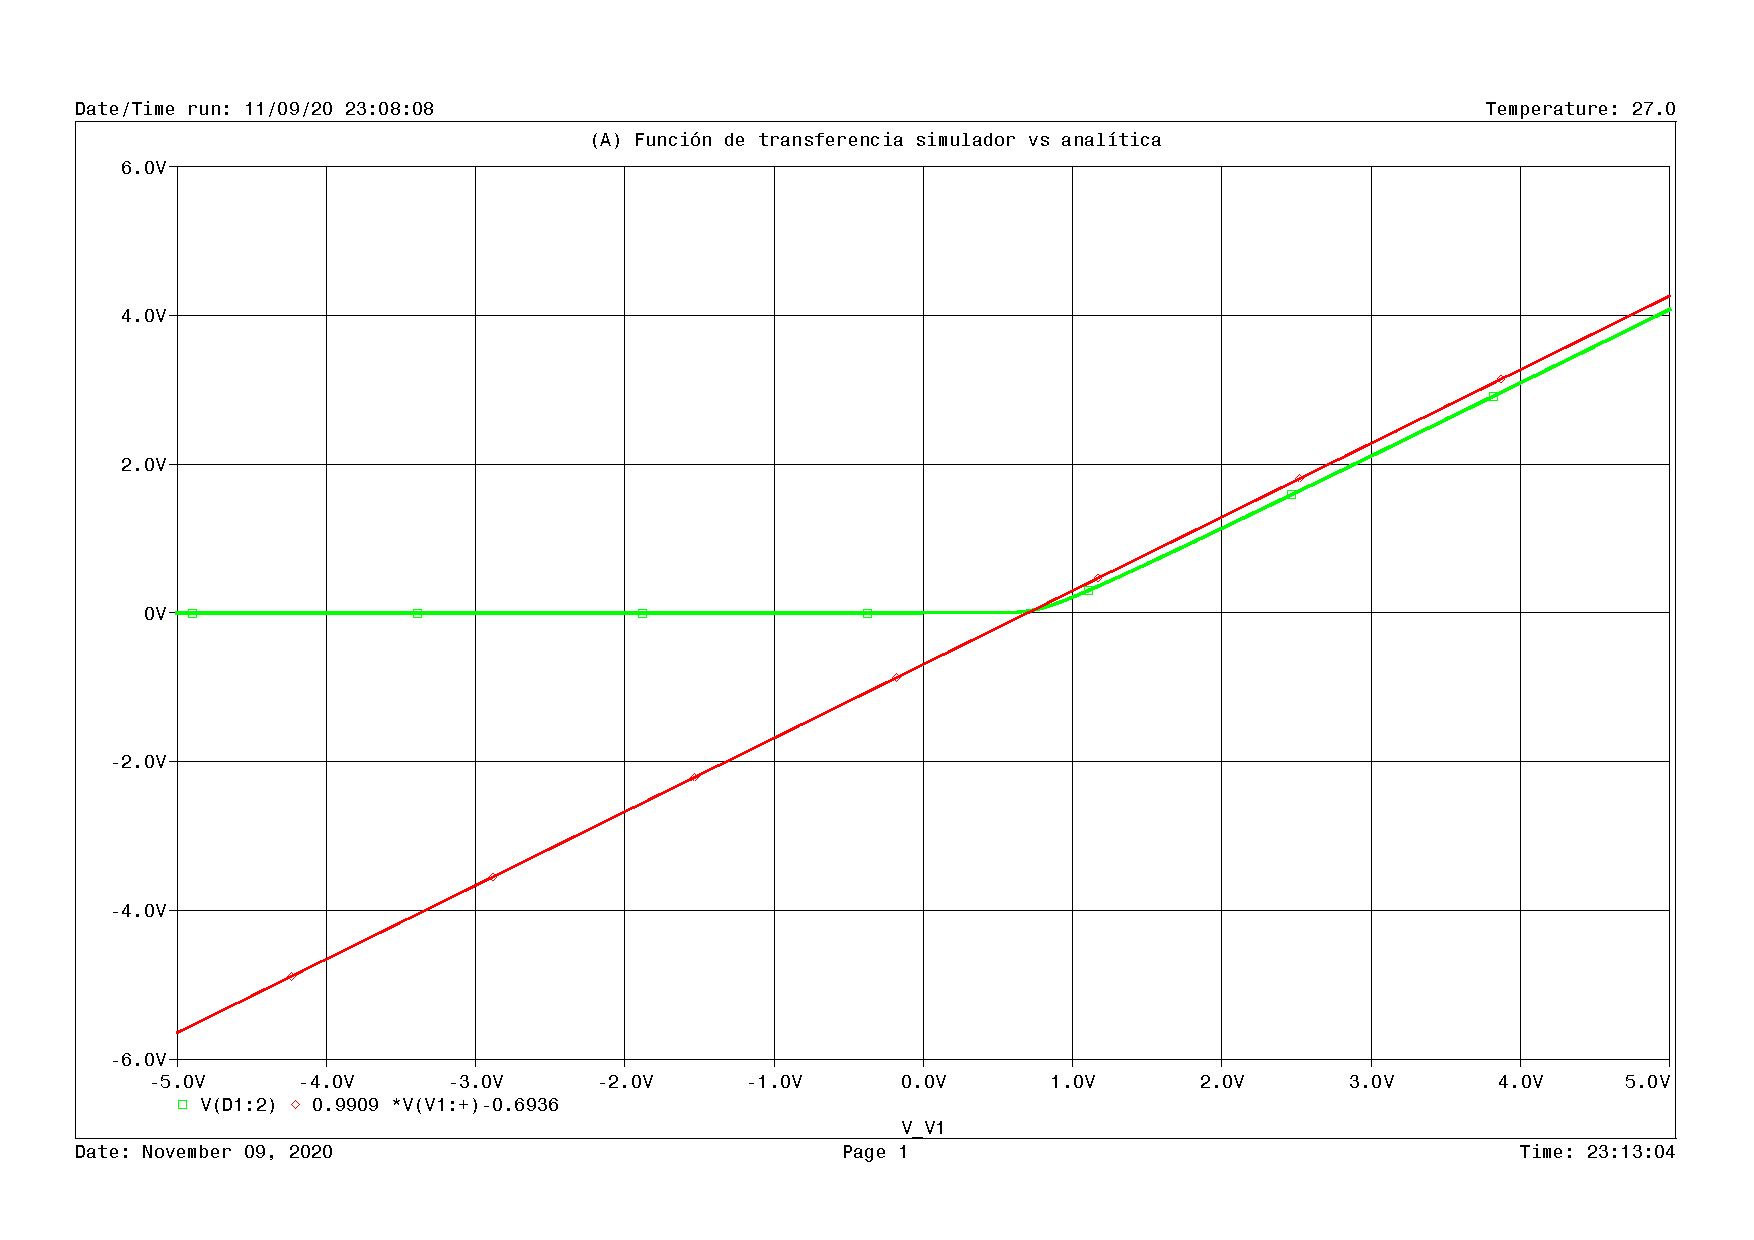
\includegraphics[scale=0.5]{images/compative_transfer.pdf}
\caption{Función de transferencia simulador vs. modelo aproximado}
\label{transfer_function_comparative}
\end{figure}

Como podemos ver en la imagen los resultados son bastante aproximados,
con una diferencia de 0.18 voltios. No debemos olvidar que la
recta (línea roja) es acotada su zona de trabajo con $x \in
[\nc{7}{-1},+\infty)$.

Después del análisis concluimos que tenemos un
\textbf{recortador negativo simple en serie no polarizado} es
decir que la tensión de entrada será recortada, se eliminan los
valores negativos y como no está polarizado el recorte mantiene
la curvatura de la función seno sin deformarla (esto se verá en
el apartado 3) pero el valor de la amplitud disminuye.
      
}

\mkexercise{Curva característica $V-I$ del diodo en el primer
  cuadrante; es decir, realizando un barrido en tensión
  en el rango: $0 \ V \leq V_{in} \leq 5 \
  V$. Interpretar el resultado comparándalo con la
  ecuación del diodo en el primer cuadrante.
\begin{figure}[H]
\centering  
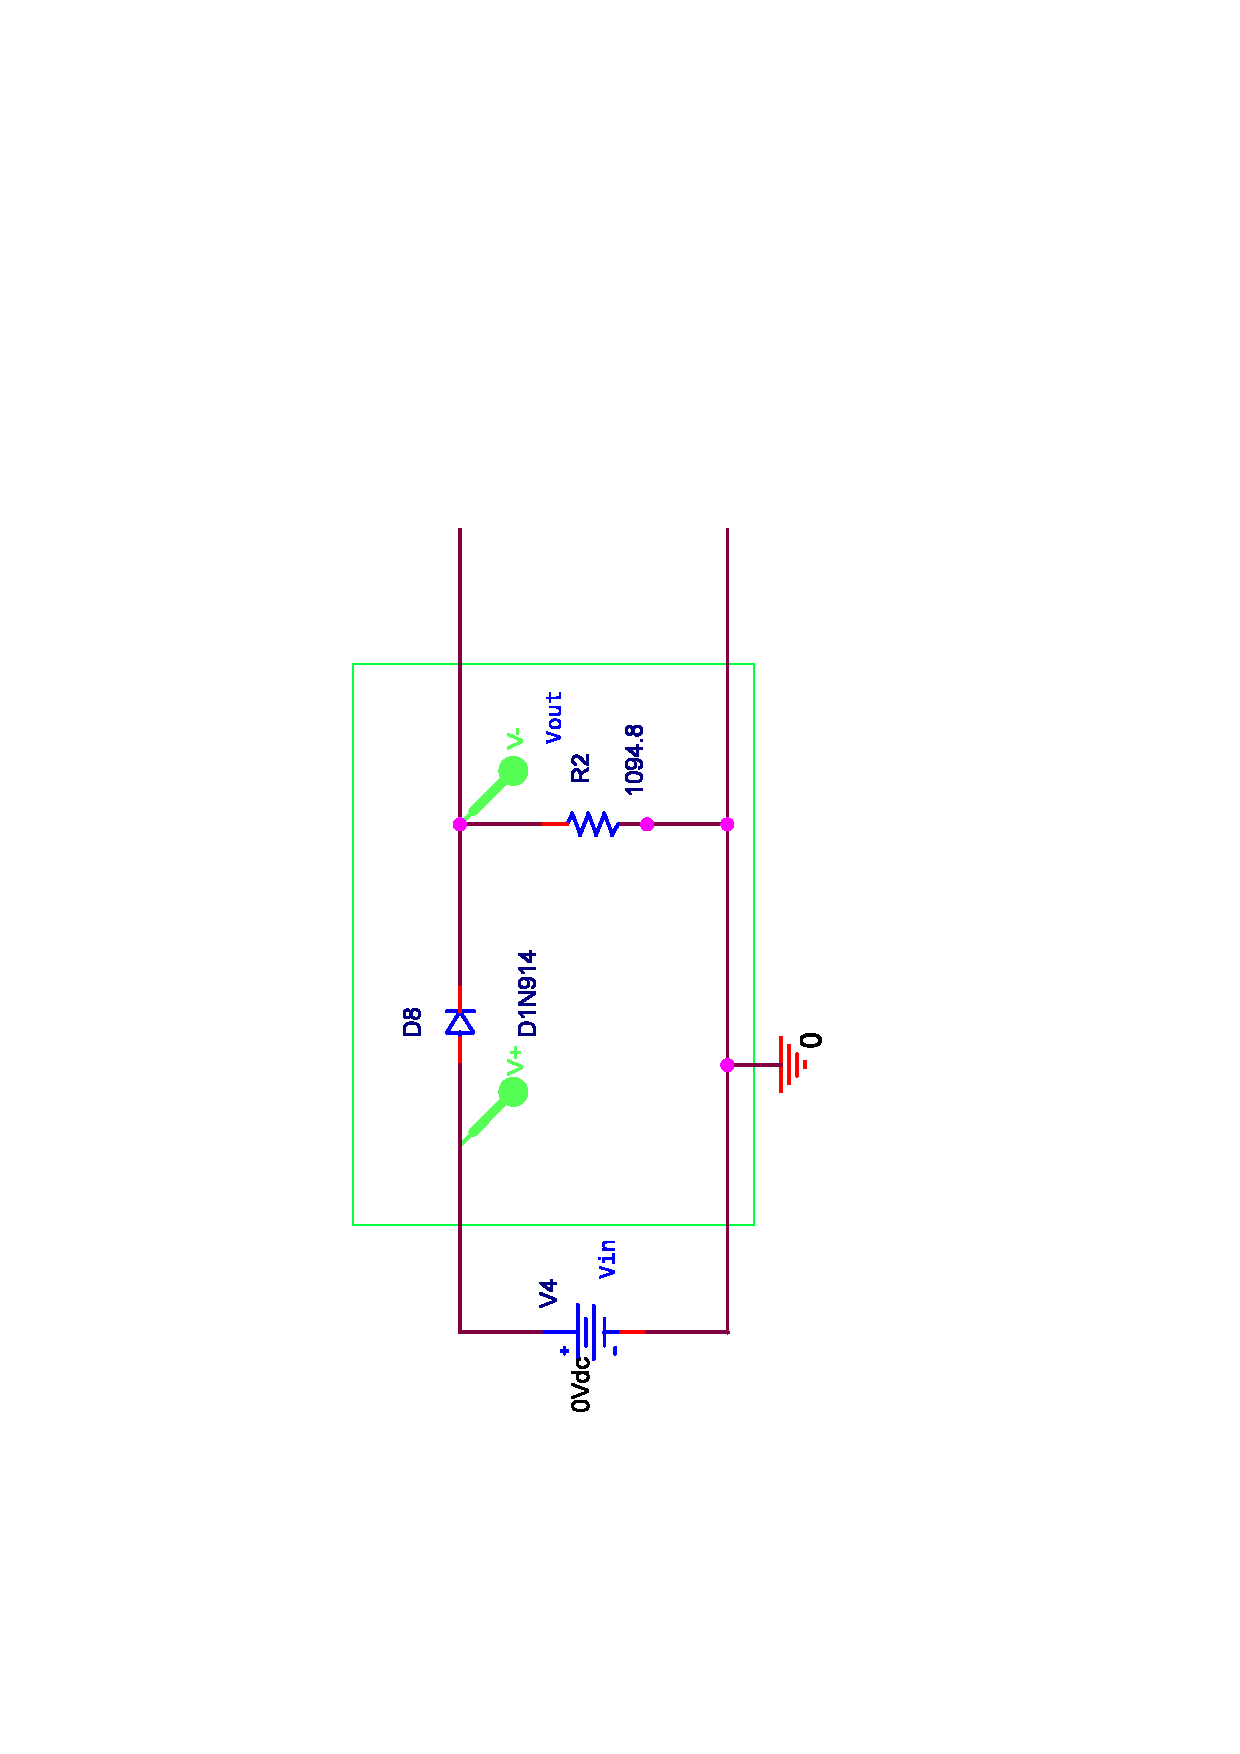
\includegraphics[clip, trim=5.7cm 5.5cm 7cm 10cm,
scale=0.75 ,angle=270]{images/ejercicio_b.pdf}
% izquierda,abajo,derecha,arriba
\caption{Circuito de estudio ``b''}
\label{circuito_estudio_b}
\end{figure}
}

\mksolution{

Usamos la ecuación del diodo de Shockley para obtener una aproximación
que podamos usar para comparar; la corriente de saturación es propia
del dispositivo, podemos encontrarla en el modelo SPICE abriendo la
libreria con el Pspice Model Editor.  Para el diodo D1N914 la $I_s$ es
$\nc{168.1}{-21} \ A$. El resto de valores son constantes y consideramos
una temperatura de $27^{\circ}C$.

  \begin{equation}
    I = I_s\left(\exp{\left(\dfrac{qV}{kT}\right)}-1\right)
  \end{equation}
  \begin{equation}
    I = \nc{168.1}{-21}\left(\exp{\left(\dfrac{V}{25 \ mV}\right)}-1\right)
  \end{equation}

  Hemos obtenido la curva analítica, ahora tenemos que obtener la
  curva de simulación.

\begin{figure}[H]
\centering  
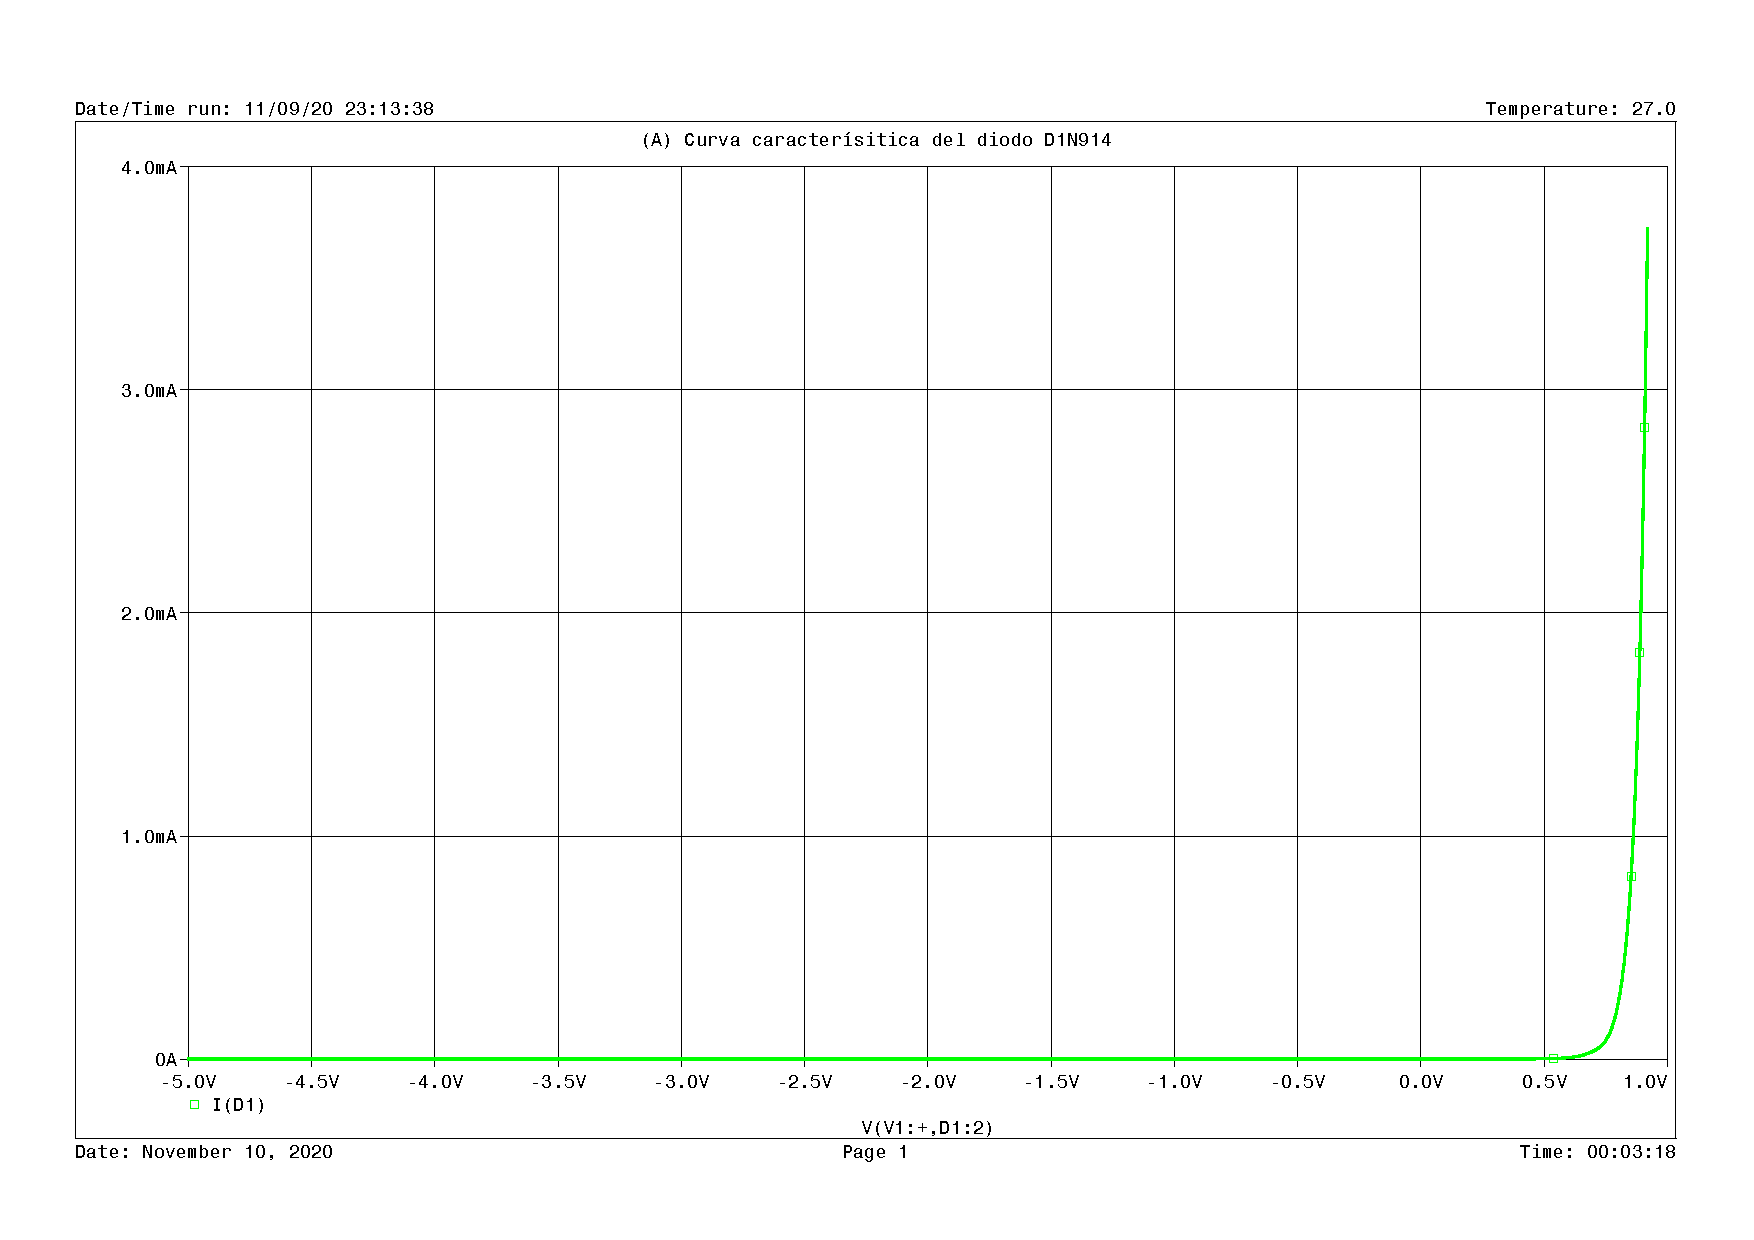
\includegraphics[scale=0.55]{images/curva_caracteristica_D1N914.pdf}
% izquierda,abajo,derecha,arriba
\caption{Curva característica del diodo D1N914}
\label{curva_Característica_del_diodo}
\end{figure}

El modelo de Shockley es bastante aproximado al del simulador, es
apreciable en el caracter exponencial que posee la ecuación, la
diferencia entre el modelo y lo que nos ofrece el simulador radica
fundamentalmente en las consideraciones de segundo y tercer orden que
hace el simulador luego habrá una ligera variación, además el modelo
de Shockley no considera la zona zener.

La mejor forma de comparar ambas curvas es usar algún
lenguaje/programa en el que podamos manejar los datos que nos
ofrece el simulador, MATALB nos permite realizar la
representación de ambas curvas y comparar su exactitud.

%%INSERTAR FIGURA MATLAB COMPARACIÓN
  
}

\mkexercise{Como señal de entrada $V_{in}$ en el circuito
   anterior, sustituir la pila por una señal senoidal
   de $5 \ V$ de amplitud y una frecuencia de $100 \ Hz$
   tal como muestra la figura:
\begin{figure}[H]
\centering
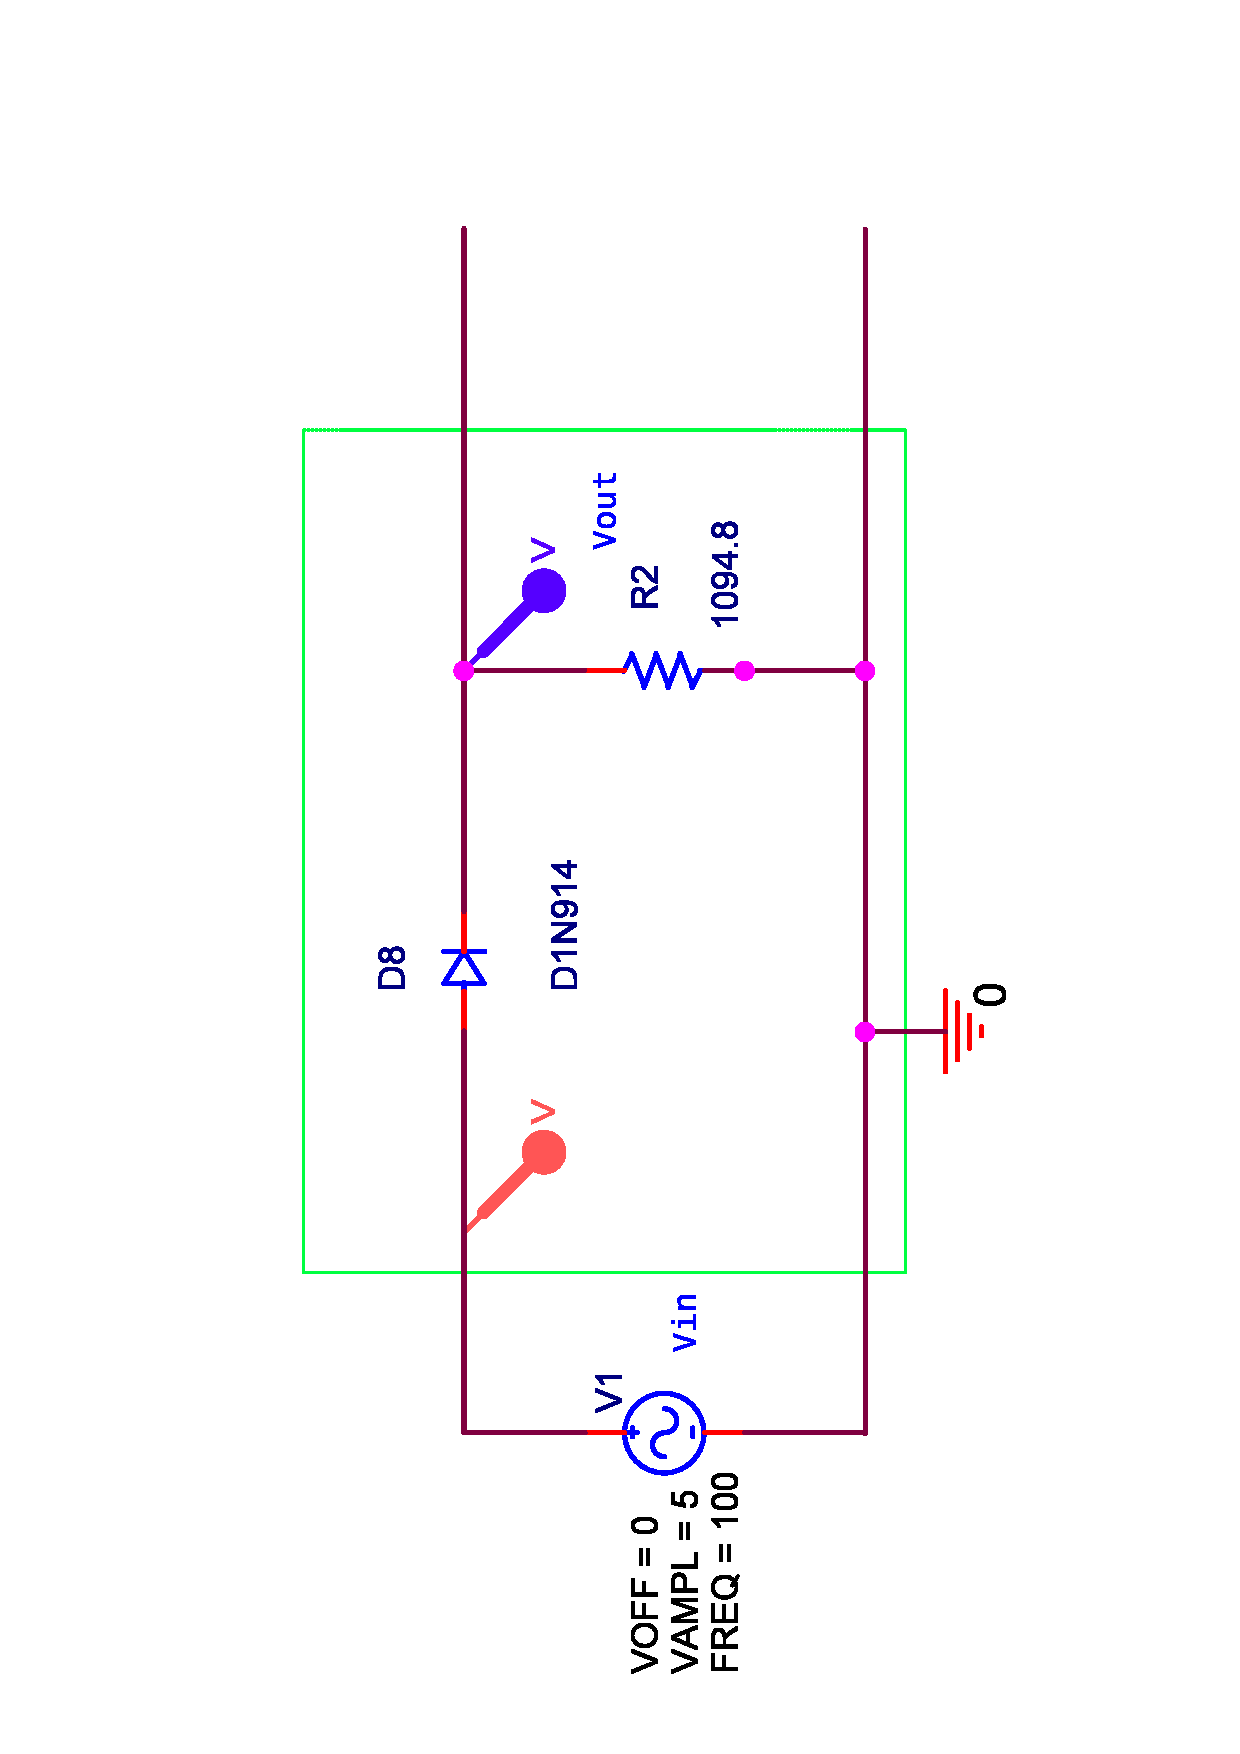
\includegraphics[clip, trim=5cm 1cm 4cm 6cm,
scale=0.46,angle=270]{images/ejercicio_c.pdf}
% izquierda,abajo,derecha,arriba
\caption{Circuito de estudio ``c''}
\label{circuito_de_estudio_c}
\end{figure}
   Realizar un análisis transitorio ``Time Domain
   (Trasient)'' para observar la señal de salida en un
   intervalo temporal de $20 \ ms$. Comparar la señal de
   entrada con la señal de salida interpretando los
   resultados y explicando la acción del diodo sobre la
   señal de salir $V_{out}$.}
\mksolution{Considerando los resultados del análisis en el apartado ``a''
  podemos determinar la salida a \textit{grosso modo}.

  Si usamos la recta de carga $0.9909V_{in}-0.6936 = V_{out}$ la
entrada máxima de $5\ V$ pasa a una salida máxima de $4.26 \ V$ luego
vemos una reducción de más de medio voltio \textit{aprox.},
considerando que el diodo no conduce en la zona negativa recortaremos
ese trozo de la señal y debemos obtener algo parecido a la figura
\ref{ref_recorte}.

  \begin{figure}[H]
    \centering
    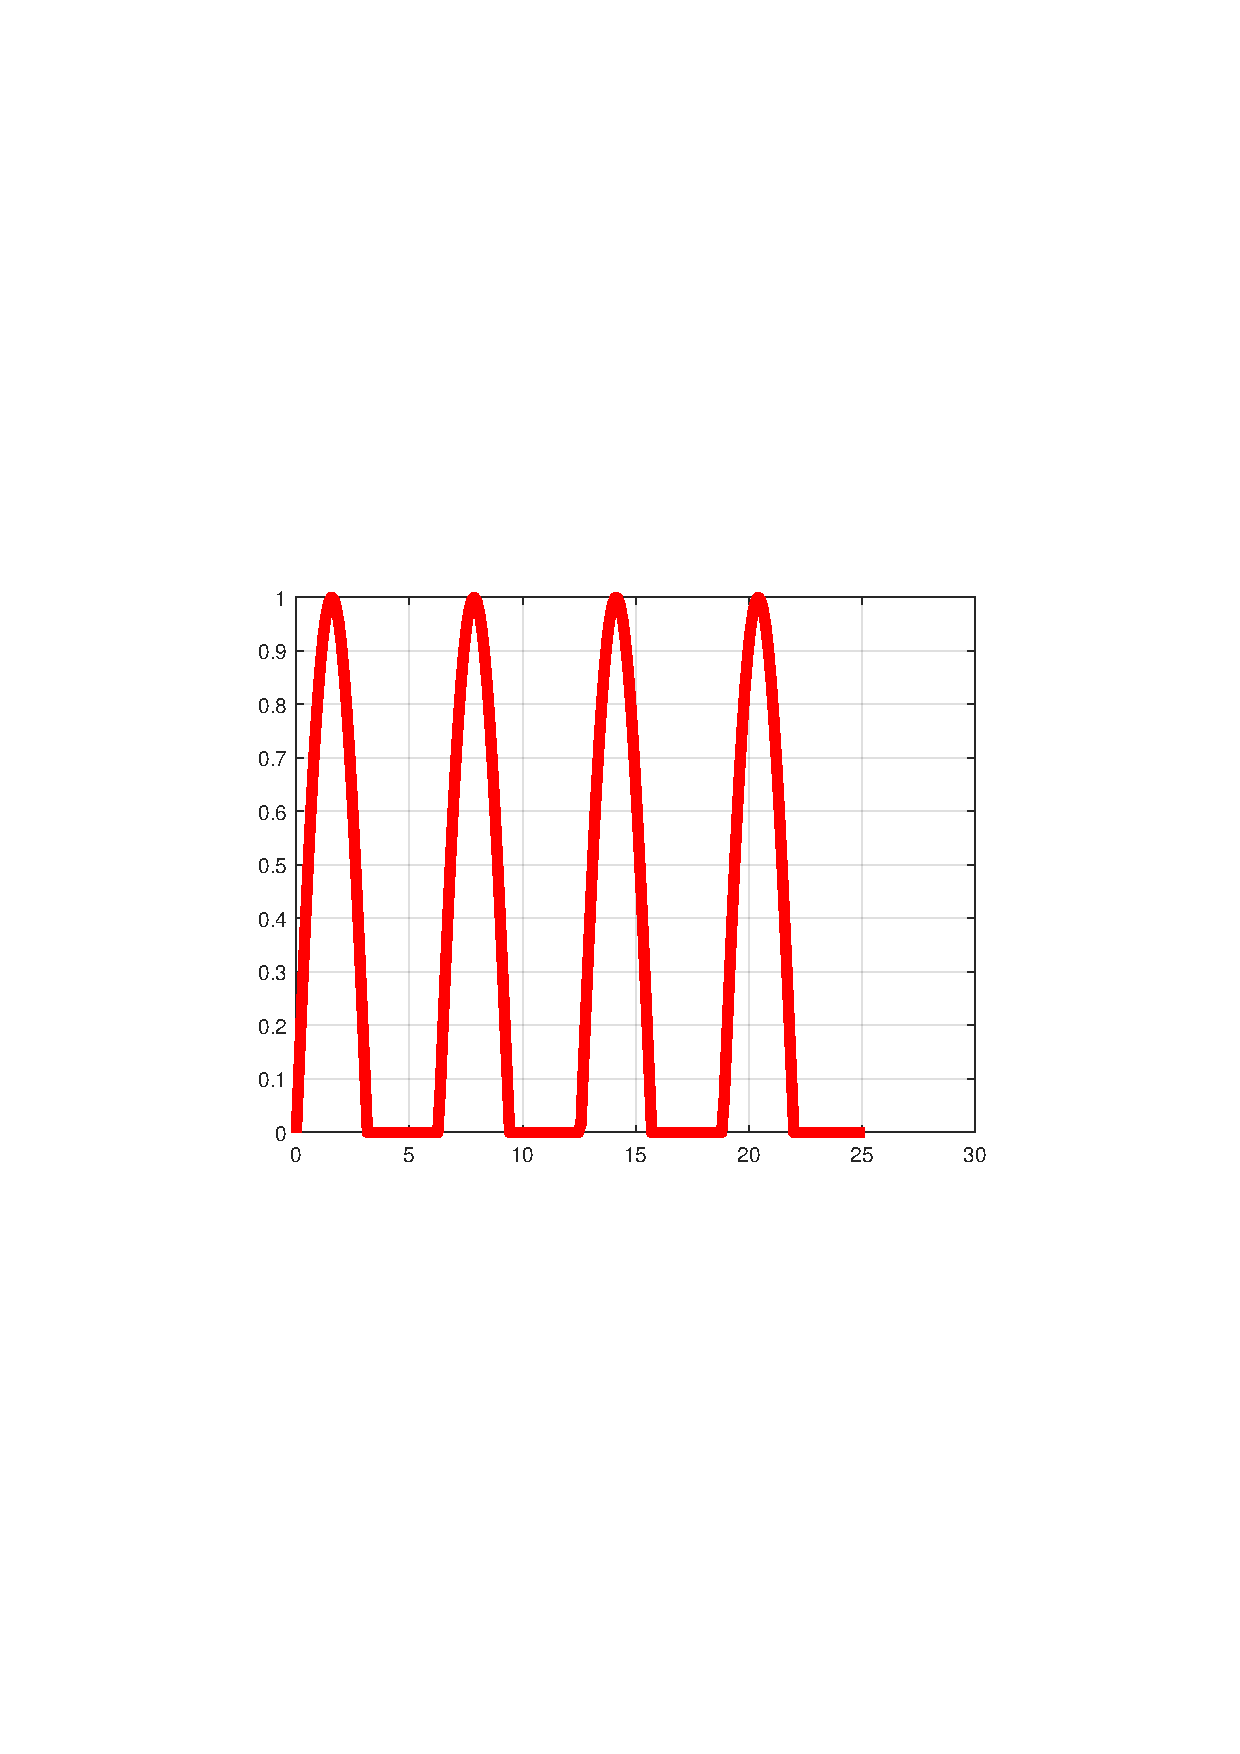
\includegraphics[clip, trim=4cm 10cm 4cm 10cm,
    scale=0.5]{images/circuito_matlab.pdf}
    \caption{Modelo de la señal de salida}
\label{ref_recorte}
\end{figure}

Vamos al simulador para confirmar los resultados esperados:

  \begin{figure}[H]
    \centering
    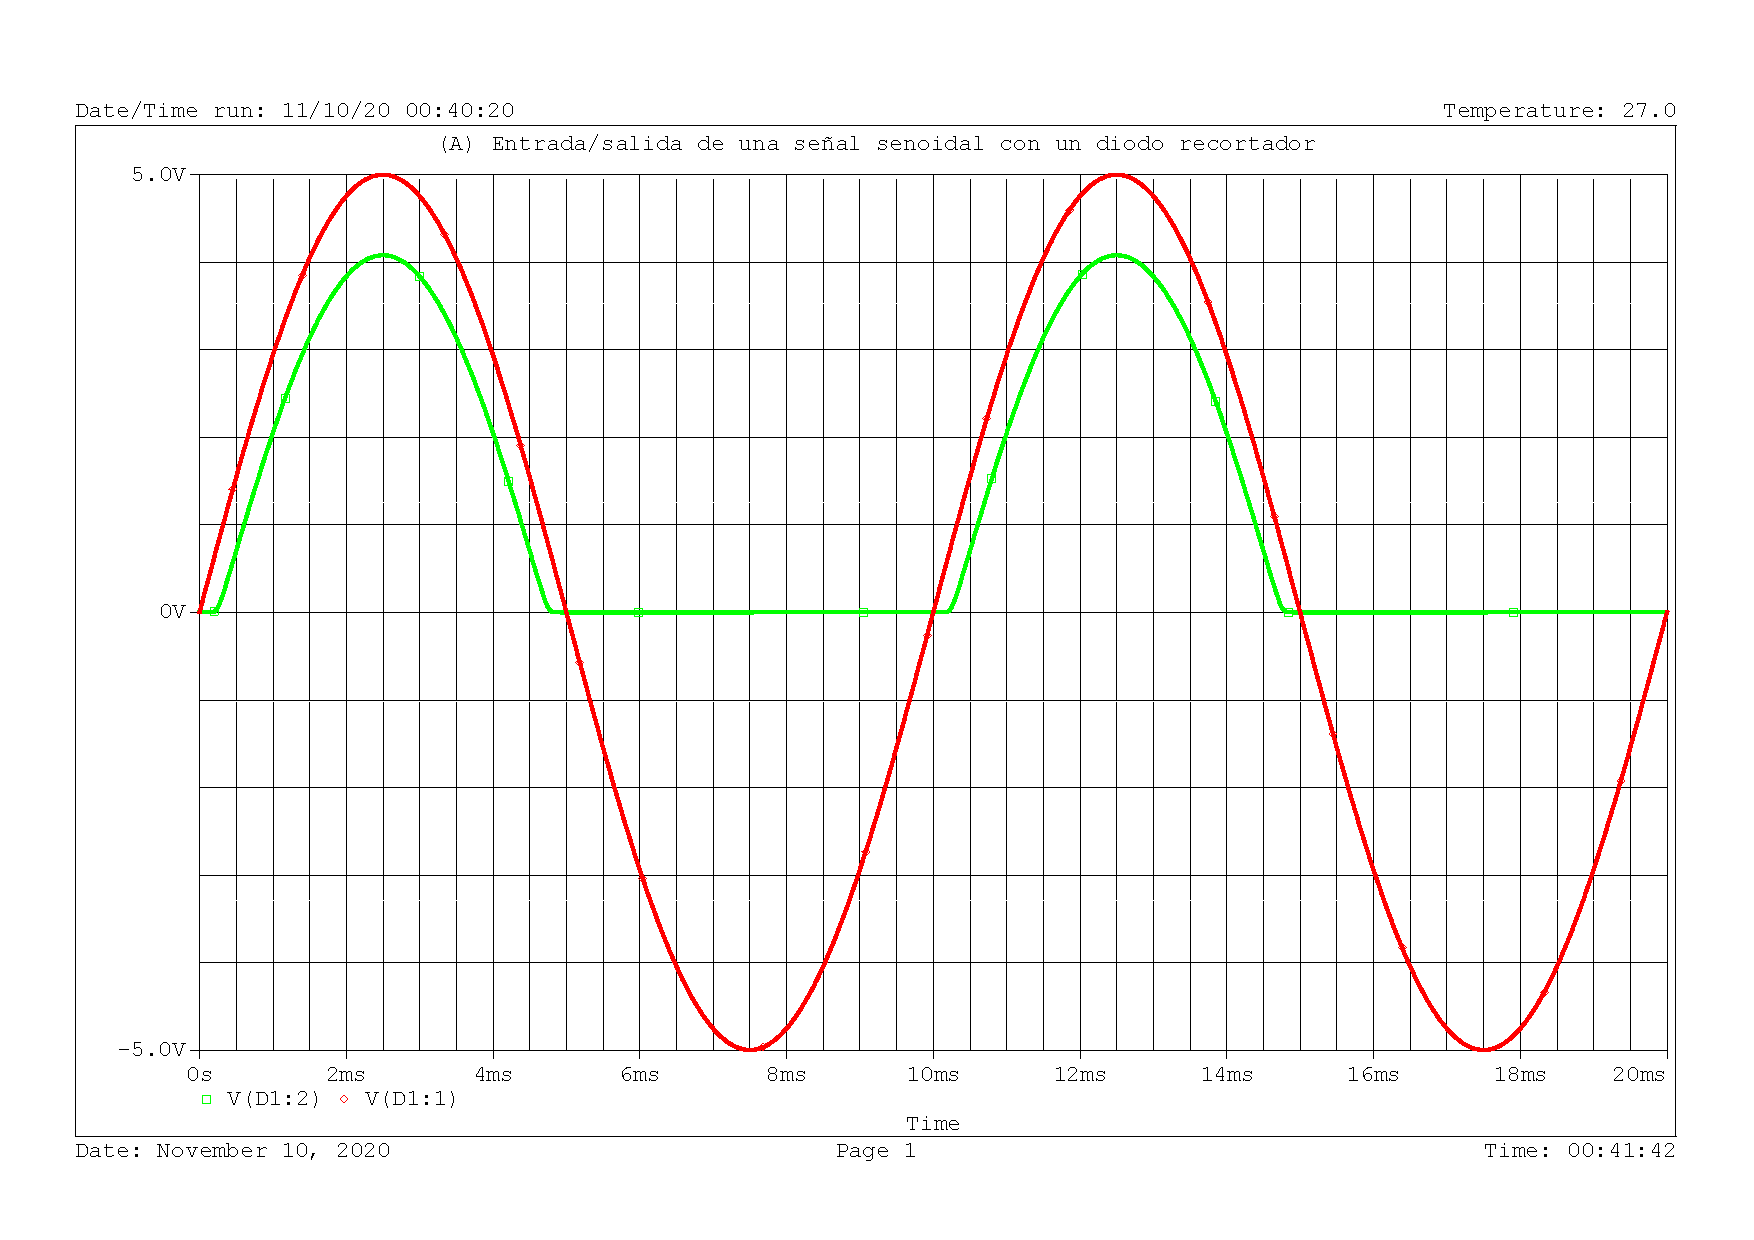
\includegraphics[scale=0.5]{images/respuesta_problema_3.pdf}
    \caption{Respuesta a una señal senoidal de $5 \ V$ a $100 \ Hz$.}
    \label{response_sen}
\label{ref_recorte}
\end{figure}

Como se puede observar en la figura \ref{response_sen} la señal de
salida ha sido recortada y limitada, concuerda con los resultados esperados.
}